\FloatBarrier
\subsection{Measured coding gain under one success rule}
\label{sec:r34}
Success is acceptable \emph{population mean full-record NMSE}, distinct
from individual-waveform or bit-perfect success. Before validation,
the phase-0 no-bit-error baseline $ d_0=\CDesignBase $ fixes
\begin{equation}
 \tau=2d_0=\CTau,\qquad
 D_{\max}=P_x\tau=\CTauMse.
 \label{eq:r34-budget}
\end{equation}
The factor two is a project preference, not a universal or perceptual limit.
Both paths retain the same threshold; the new $ p=0 $ mean $\CNewBase $
does not recalibrate it. Total error retains upstream/channel cross terms
(Eq.~\eqref{eq:r34-cross}).
The 12 R3.3 conditions plus prespecified refinements $0.002,0.004,0.005 $
are tested with 300 new Gaussian inputs, 8400 positive-$ p $ masks and 9000
path records. Whole records are the independent units; Gaussian inputs
are shared across probabilities and layouts, so curves are dependent.
\begin{equation}
 \text{Gaussian: }(1,3,1,5,r),\qquad
 \text{BSC: }(2,3,1,c,r,\ell),\quad r=0,\ldots,299,\quad\ell=0,1.
 \label{eq:r34-paths}
\end{equation}
The earlier nested-bank variance estimate plans 300 records with half-width
target $0.1\tau $ near the two design boundaries; no validation result
changes the count. Approximate Bonferroni t/CLT intervals cover the finite
30-mean family (Appendix~\ref{app:statistics}), not a continuous-$ p $ band
or individual future records. The common rule and requested gain set are
\begin{equation}
 \operatorname{status}=
 \begin{cases}
 \mathrm{pass},&U\le\tau,\\
 \mathrm{fail},&L>\tau,\\
 \mathrm{inconclusive},&\text{otherwise}.
 \end{cases}
 \label{eq:r34-decision}
\end{equation}
\begin{equation}
 \mathcal G_{\rm tested}=
 \{p:\ U_{\rm coded}(p)\le\tau
          \ \text{and}\ L_{\rm uncoded}(p)>\tau\}.
 \label{eq:r34-gain}
\end{equation}

\begin{table}[htbp]
 \centering\small
 \caption{Independent NMSE means and approximate 30-family intervals, 300 records per path/condition. Gain means coded pass and uncoded fail at the same fixed threshold; decisions use unrounded CSV.}
 \label{tab:r34-quality}
 \begin{tabular}{rlll}
\toprule
$p$ & Uncoded mean [adjusted CI] & Hamming mean [adjusted CI] & Gain \\
\midrule
$0$ & 0.0291 [0.0289,0.0292] & 0.0291 [0.0289,0.0292] & no \\
$0.0001$ & 0.0873 [0.0825,0.0922] & 0.0292 [0.0289,0.0294] & yes \\
$p_{\rm ID}$ & 0.1516 [0.1449,0.1582] & 0.0292 [0.0290,0.0294] & yes \\
$0.0003$ & 0.2068 [0.1990,0.2146] & 0.0292 [0.0290,0.0295] & yes \\
$0.001$ & 0.6223 [0.6087,0.6360] & 0.0333 [0.0321,0.0346] & yes \\
$0.002$ & 1.2219 [1.2007,1.2431] & 0.0436 [0.0416,0.0457] & yes \\
$0.003$ & 1.7901 [1.7653,1.8149] & 0.0638 [0.0603,0.0673] & no \\
$0.004$ & 2.3823 [2.3534,2.4112] & 0.0922 [0.0877,0.0967] & no \\
$0.005$ & 2.9606 [2.9275,2.9936] & 0.1196 [0.1143,0.1249] & no \\
$0.01$ & 5.8943 [5.8475,5.9411] & 0.3970 [0.3866,0.4074] & no \\
$0.03$ & 17.2616 [17.1866,17.3365] & 3.1534 [3.1229,3.1839] & no \\
$0.1$ & 53.2739 [53.1572,53.3906] & 27.3053 [27.2175,27.3931] & no \\
$0.2$ & 94.8705 [94.7203,95.0206] & 75.2253 [75.0877,75.3630] & no \\
$0.3$ & 124.6956 [124.5513,124.8398] & 115.9078 [115.7615,116.0540] & no \\
$0.5$ & 148.9787 [148.8422,149.1151] & 149.0071 [148.8766,149.1377] & no \\
\bottomrule
\end{tabular}

 
 
\end{table}


\begin{figure}[htbp]
 \centering
 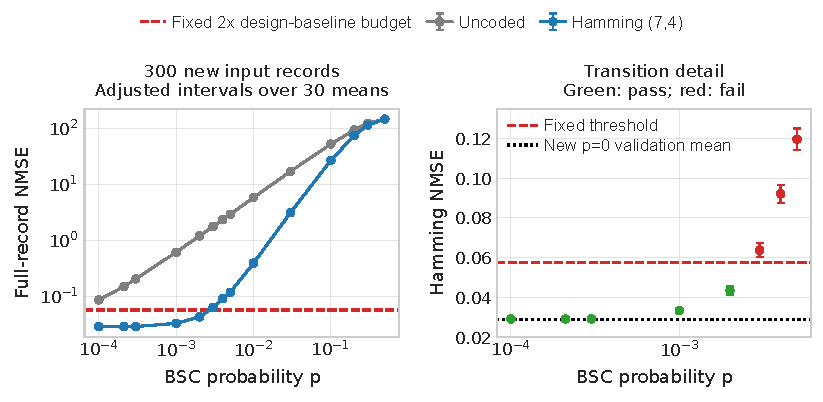
\includegraphics[width=.86\linewidth]{supporting/publication_r34_quality_gain_horizontal.pdf}
 \caption{Coded/uncoded mean quality over the full envelope (left) and the coded transition detail (right). Error bars use the frozen 30-mean family; the threshold is fixed before validation.}
 \label{fig:r34-quality}
\end{figure}

The primary measured gain is
\begin{equation}
 \boxed{\mathcal G_{\rm tested}
   =\{0.0001,\ p_{\rm ID},\ 0.0003,\ 0.001,\ 0.002\}}.
 \label{eq:r34-result}
\end{equation}
At the anchor point, coded/uncoded mean NMSE is
$\CPersonalCoded/\CPersonalUncoded $; the respective intervals lie below
and above $\tau $. The largest coded passing test point is 0.002; 0.003
fails. Uncoded $ p=0 $ passes, whereas $10^{-4}$ fails. These are tested
brackets, not exact continuous crossings. At higher $ p $ both fail quality
even where coding still reduces BER. The ancillary mean paired
reconstruction-error gain is \CPersonalGainDb\,dB, pointwise 95 \%
interval $[\CPersonalGainLow,\CPersonalGainHigh]$; it is not an $ E_b/N_0 $
gain or the log ratio of two mean MSEs.

\paragraph{Three meanings of success and the resource cost.}

\begin{figure}[htbp]
 \centering
 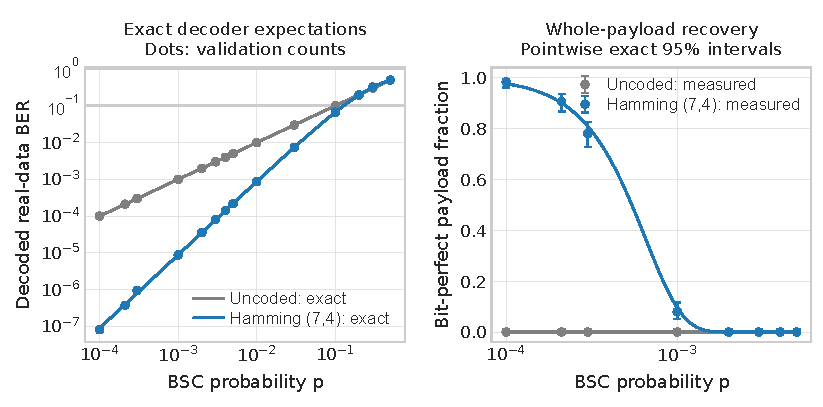
\includegraphics[width=.86\linewidth]{supporting/publication_r34_bit_recovery_horizontal.pdf}
 \caption{BER versus exact decoder expectations (left); complete 448000-bit payload recovery with pointwise 95\% proportion intervals (right). Zero BER counts are omitted from the log axis.}
 \label{fig:r34-bits}
\end{figure}

At $ p=0.002 $ the coded mean passes, 264/300 individual waveforms pass,
and 0/300 complete payloads are bit-perfect. At the anchor point all 300
coded waveforms pass but only \CPerfectPersonal/300 payloads are perfect;
both uncoded counts are zero. The coded perfect-payload estimate is
 \CPerfectPersonalPercent\%, pointwise exact 95 \% interval
$[\CPerfectPersonalLow,\CPerfectPersonalHigh]\%$; its theoretical value is
 \CPerfectPersonalTheory\% (Eq.~\eqref{eq:r34-payload}).
These digital-message probabilities differ from the 30-family waveform
mean intervals. The exact BER/block laws describe actual independent BSC
flips, not an imposed single-flip experiment.

Prespecified threshold factors 1.5, 2, 4 retain exclusive gain at $ p_{\rm ID}$,
0.0003 and 0.001. Other classifications can change: an interval crossing
the threshold remains inconclusive, not silently a pass.
The coded stream sends 784000 bits versus 448000 uncoded: 75 \% overhead,
392 versus 224 kbit/s, within the twofold budget. Equal $ p $ is not equal
traffic or energy. Alternative-method replay (Section~\ref{sec:r61})
verifies all 9000 paths/decisions within MSE $4.27\times10^{-14}$;
no overload was observed.
This establishes a conditional result for the supplied record, fixed
anchor SNR, framing and budget, rather than universal code optimality.
